% Options for packages loaded elsewhere
\PassOptionsToPackage{unicode}{hyperref}
\PassOptionsToPackage{hyphens}{url}
%
\documentclass[]{article}
% \author{}
% \date{}

\usepackage{amsmath,amssymb}
\usepackage{lmodern}
\usepackage{iftex}
\ifPDFTeX
  \usepackage[T1]{fontenc}
  \usepackage[utf8]{inputenc}
  \usepackage{textcomp} % provide euro and other symbols
\else % if luatex or xetex
  \usepackage{unicode-math}
  \defaultfontfeatures{Scale=MatchLowercase}
  \defaultfontfeatures[\rmfamily]{Ligatures=TeX,Scale=1}
\fi
% Use upquote if available, for straight quotes in verbatim environments
\IfFileExists{upquote.sty}{\usepackage{upquote}}{}
\IfFileExists{microtype.sty}{% use microtype if available
  \usepackage[]{microtype}
  \UseMicrotypeSet[protrusion]{basicmath} % disable protrusion for tt fonts
}{}
\makeatletter
\@ifundefined{KOMAClassName}{% if non-KOMA class
  \IfFileExists{parskip.sty}{%
    \usepackage{parskip}
  }{% else
    \setlength{\parindent}{0pt}
    \setlength{\parskip}{6pt plus 2pt minus 1pt}}
}{% if KOMA class
  \KOMAoptions{parskip=half}}
\makeatother
\usepackage{xcolor}
\IfFileExists{xurl.sty}{\usepackage{xurl}}{} % add URL line breaks if available
\IfFileExists{bookmark.sty}{\usepackage{bookmark}}{\usepackage{hyperref}}
\hypersetup{
  hidelinks,
  pdfcreator={LaTeX via pandoc}}
\urlstyle{same} % disable monospaced font for URLs
\usepackage{color}
\usepackage{fancyvrb}
\newcommand{\VerbBar}{|}
\newcommand{\VERB}{\Verb[commandchars=\\\{\}]}
\DefineVerbatimEnvironment{Highlighting}{Verbatim}{commandchars=\\\{\}}
% Add ',fontsize=\small' for more characters per line
\newenvironment{Shaded}{}{}
\newcommand{\AlertTok}[1]{\textcolor[rgb]{1.00,0.00,0.00}{\textbf{#1}}}
\newcommand{\AnnotationTok}[1]{\textcolor[rgb]{0.38,0.63,0.69}{\textbf{\textit{#1}}}}
\newcommand{\AttributeTok}[1]{\textcolor[rgb]{0.49,0.56,0.16}{#1}}
\newcommand{\BaseNTok}[1]{\textcolor[rgb]{0.25,0.63,0.44}{#1}}
\newcommand{\BuiltInTok}[1]{#1}
\newcommand{\CharTok}[1]{\textcolor[rgb]{0.25,0.44,0.63}{#1}}
\newcommand{\CommentTok}[1]{\textcolor[rgb]{0.38,0.63,0.69}{\textit{#1}}}
\newcommand{\CommentVarTok}[1]{\textcolor[rgb]{0.38,0.63,0.69}{\textbf{\textit{#1}}}}
\newcommand{\ConstantTok}[1]{\textcolor[rgb]{0.53,0.00,0.00}{#1}}
\newcommand{\ControlFlowTok}[1]{\textcolor[rgb]{0.00,0.44,0.13}{\textbf{#1}}}
\newcommand{\DataTypeTok}[1]{\textcolor[rgb]{0.56,0.13,0.00}{#1}}
\newcommand{\DecValTok}[1]{\textcolor[rgb]{0.25,0.63,0.44}{#1}}
\newcommand{\DocumentationTok}[1]{\textcolor[rgb]{0.73,0.13,0.13}{\textit{#1}}}
\newcommand{\ErrorTok}[1]{\textcolor[rgb]{1.00,0.00,0.00}{\textbf{#1}}}
\newcommand{\ExtensionTok}[1]{#1}
\newcommand{\FloatTok}[1]{\textcolor[rgb]{0.25,0.63,0.44}{#1}}
\newcommand{\FunctionTok}[1]{\textcolor[rgb]{0.02,0.16,0.49}{#1}}
\newcommand{\ImportTok}[1]{#1}
\newcommand{\InformationTok}[1]{\textcolor[rgb]{0.38,0.63,0.69}{\textbf{\textit{#1}}}}
\newcommand{\KeywordTok}[1]{\textcolor[rgb]{0.00,0.44,0.13}{\textbf{#1}}}
\newcommand{\NormalTok}[1]{#1}
\newcommand{\OperatorTok}[1]{\textcolor[rgb]{0.40,0.40,0.40}{#1}}
\newcommand{\OtherTok}[1]{\textcolor[rgb]{0.00,0.44,0.13}{#1}}
\newcommand{\PreprocessorTok}[1]{\textcolor[rgb]{0.74,0.48,0.00}{#1}}
\newcommand{\RegionMarkerTok}[1]{#1}
\newcommand{\SpecialCharTok}[1]{\textcolor[rgb]{0.25,0.44,0.63}{#1}}
\newcommand{\SpecialStringTok}[1]{\textcolor[rgb]{0.73,0.40,0.53}{#1}}
\newcommand{\StringTok}[1]{\textcolor[rgb]{0.25,0.44,0.63}{#1}}
\newcommand{\VariableTok}[1]{\textcolor[rgb]{0.10,0.09,0.49}{#1}}
\newcommand{\VerbatimStringTok}[1]{\textcolor[rgb]{0.25,0.44,0.63}{#1}}
\newcommand{\WarningTok}[1]{\textcolor[rgb]{0.38,0.63,0.69}{\textbf{\textit{#1}}}}
\usepackage{longtable,booktabs,array}
\usepackage{calc} % for calculating minipage widths
% Correct order of tables after \paragraph or \subparagraph
\usepackage{etoolbox}
\makeatletter
\patchcmd\longtable{\par}{\if@noskipsec\mbox{}\fi\par}{}{}
\makeatother
% Allow footnotes in longtable head/foot
\IfFileExists{footnotehyper.sty}{\usepackage{footnotehyper}}{\usepackage{footnote}}
\makesavenoteenv{longtable}
\usepackage{graphicx}
\makeatletter
\def\maxwidth{\ifdim\Gin@nat@width>\linewidth\linewidth\else\Gin@nat@width\fi}
\def\maxheight{\ifdim\Gin@nat@height>\textheight\textheight\else\Gin@nat@height\fi}
\makeatother
% Scale images if necessary, so that they will not overflow the page
% margins by default, and it is still possible to overwrite the defaults
% using explicit options in \includegraphics[width, height, ...]{}
\setkeys{Gin}{width=\maxwidth,height=\maxheight,keepaspectratio}
% Set default figure placement to htbp
\makeatletter
\def\fps@figure{htbp}
\makeatother
\setlength{\emergencystretch}{3em} % prevent overfull lines
\providecommand{\tightlist}{%
  \setlength{\itemsep}{0pt}\setlength{\parskip}{0pt}}
\setcounter{secnumdepth}{-\maxdimen} % remove section numbering
\ifLuaTeX
  \usepackage{selnolig}  % disable illegal ligatures
\fi

\begin{document}

\hypertarget{tiny-vector-graphics-specification}{%
\section{Tiny Vector Graphics
(Specification)}\label{tiny-vector-graphics-specification}}

\textbf{Abstract:} The tiny vector graphics format is a binary file
format that encodes a list of vector graphic primitives. It is tailored
to have a tiny memory footprint and simple implementations, while
lifting small file size over encoding simplicity.

\hypertarget{introduction}{%
\subsection{Introduction}\label{introduction}}

\hypertarget{why-a-new-format}{%
\subsubsection{Why a new format}\label{why-a-new-format}}

SVG is the status quo widespread vector format. Every program can kinda
use it and can probably render it right to some extend. The problem is
that SVG is a horribly large specification, it is based on XML and
provides not only vector graphics, but also a full suite for animation
and JavaScript scripting. Implementing a new SVG renderer from scratch
is a tremendous amount of work, and it is hard to get it done right.

Quoting the \href{https://de.wikipedia.org/wiki/Scalable_Vector_Graphics}{german Wikipedia}:

\begin{quote}
Praktisch alle relevanten Webbrowser können einen Großteil des
Sprachumfangs darstellen.\\
Virtually all relevant web browsers can display a large part of the
language range.
\end{quote}

The use of XML bloats the files by a huge magnitude and doesn't provide
a efficient encoding, thus a lot of websites and applications ship files
that are not encoded optimally. Also SVG allows several ways of
achieving the same thing, and can be seen more as a intermediate format
for editing as for final encoding.

TinyVG was created to adress most of these problems, trying to achieve a
balance between flexibility and file size, while keeping file size as
the more important priority.

\hypertarget{features}{%
\subsubsection{Features}\label{features}}

\begin{itemize}
\tightlist
\item
  Binary encoding
\item
  Support of the most common 2D vector primitives

  \begin{itemize}
  \tightlist
  \item
    Paths
  \item
    Polygons
  \item
    Rectangles
  \item
    Lines
  \end{itemize}
\item
  3 different fill styles

  \begin{itemize}
  \tightlist
  \item
    Flat color
  \item
    Linear 2-point gradient
  \item
    Radial 2-point gradient
  \end{itemize}
\item
  Dense encoding, there are near zero padding bits and every byte is
  used as good as possible.
\end{itemize}

\hypertarget{format}{%
\subsection{Format}\label{format}}

TVG files are roughly structured like this:

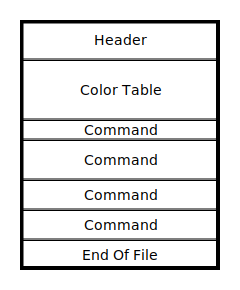
\includegraphics{graphics/overview.pdf}

Files are made up of a header, followed by a color lookup table and a
sequence of commands terminated by a \emph{end of file} command.

Concrete color values will only be present in the color table. After the
table, only indices into the color table are used to define color
values. This allows to keep the format small, as the first 128 colors in
the vector data are encoded as only a single byte, even if the color
format uses 16 bytes per color. This means in the worst case, we add a
single byte to the size of a color that is only used once, but colors
that are common in the file will be encoded as a single byte per use +
one time overhead. This encoding scheme was chosen as a vector graphic
typically doesn't use as much different colors as bitmap graphics and
thus can be encoded more optimally.

\textbf{NOTE:} The following documentation uses a tabular style to
document structures. All integers are assumed to be encoded in
little-endian byte order if not specified otherwise. The \emph{Type}
column of each structure definition uses a Zig notation for types and
the fields have no padding bits inbetween. If a field does not align to
a byte boundary, the next field will be offset into the byte by the
current fields bit offset + bit size. This means, that two consecutive
fields \textbf{a} (\texttt{u3}) and \textbf{b} (\texttt{u5}) can be
extracted from the byte by using
\texttt{(byte\ \&\ 0x7)\ \textgreater{}\textgreater{}\ 0} for \textbf{a}
and \texttt{(byte\ \&\ 0x1F)\ \textgreater{}\textgreater{}\ 3} for
\textbf{b}.

\hypertarget{coordinate-system}{%
\subsubsection{Coordinate system}\label{coordinate-system}}

TinyVG uses the 2-dimensional
\href{https://en.wikipedia.org/wiki/Cartesian_coordinate_system}{Cartesian
coordinate system} with X being the positive horizontal distance to the
origin and Y being the negative vertical distance to the origin. This
means that X is going right, while Y is going down, to match the
coordinate system of several other image formats:

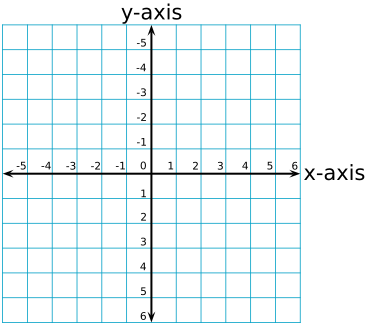
\includegraphics{graphics/coordinates.pdf}

\hypertarget{header}{%
\subsubsection{Header}\label{header}}

Each TVG file starts with a header defining some global values for the
file like scale and image size. The header is always at offset 0 in a
file.

\begin{longtable}[]{@{}lll@{}}
\toprule
Field & Type & Description \\
\midrule
\endhead
magic & \texttt{{[}2{]}u8} & Must be \texttt{\{\ 0x72,\ 0x56\ \}} \\
version & \texttt{u8} & Must be \texttt{1}. For future versions, this
field might decide how the rest of the format looks like. \\
scale & \texttt{u4} & Defines the number of fraction bits in a
\protect\hyperlink{units}{\texttt{Unit}} value. \\
color\_encoding & \texttt{u2} & Defines the type of color information
that is used in the \protect\hyperlink{color-table}{color table}. \\
coordinate\_range & \texttt{u2} & Defines the number of total bits in a
\protect\hyperlink{units}{\texttt{Unit}} value and thus the overall
precision of the file. \\
width & \texttt{u8}, \texttt{u16} or \texttt{u32} & Encodes the maximum
width of the output file in pixels. A value of 0 indicates that the
image has the maximum possible width. The size of this field depends on
the coordinate range field. \\
height & \texttt{u8}, \texttt{u16} or \texttt{u32} & Encodes the maximum
height of the output file in pixels. A value of 0 indicates that the
image has the maximum possible height. The size of this field depends on
the coordinate range field. \\
color\_count & \texttt{VarUInt} & The number of colors in the
\protect\hyperlink{color-table}{color table}. \\
\bottomrule
\end{longtable}

\hypertarget{color-encoding}{%
\paragraph{Color Encoding}\label{color-encoding}}

The color encoding defines which format the colors in the color table
will have:

\begin{longtable}[]{@{}lll@{}}
\toprule
Value & Enumeration & Description \\
\midrule
\endhead
0 & RGBA 8888 & Each color is a 4-tuple (red, green ,blue, alpha) of
bytes with the color channels encoded in sRGB and the alpha as linear
alpha. \\
1 & RGB 565 & Each color is encoded as a 3-tuple (red, green, blue) with
16 bit per color. While red and blue both use 5 bit, the green channel
uses 6 bit. red uses bit range 0...4, green bits 5...10 and blue bits
11...15. \\
2 & RGBA F32 & Each color is a 4-tuple (red, green ,blue, alpha) of
binary32 IEEE 754 floating point value with the color channels encoded
in sRGB and the alpha as linear alpha. A color value of \texttt{1.0} is
full brightness, while a value of \texttt{0.0} is zero brightness. \\
3 & Custom & The custom color encoding is \emph{defined undefined}. The
information how these colors are encoded must be implemented via
external means. \\
\bottomrule
\end{longtable}

\hypertarget{coordinate-range}{%
\paragraph{Coordinate Range}\label{coordinate-range}}

The coordinate range defines how many bits a
\protect\hyperlink{units}{\texttt{Unit}} value uses:

\begin{longtable}[]{@{}lll@{}}
\toprule
Value & Enumeration & Description \\
\midrule
\endhead
0 & Default & Each \texttt{Unit} takes up 8 bit. \\
1 & Reduced & Each \texttt{Unit} takes up 16 bit. \\
2 & Enhanced & Each \texttt{Unit} takes up 32 bit. \\
\bottomrule
\end{longtable}

\hypertarget{varuint}{%
\paragraph{\texorpdfstring{\texttt{VarUInt}}{VarUInt}}\label{varuint}}

This type is used to encode 32 bit unsigned integers while keeping the
number of bytes low. It is encoded as a variable-sized integer that uses
7 bit per byte for integer bits and the 7th bit to encode that there is
"more bits available".

The integer is still built as a little-endian, so the first byte will
always encode bits 0\ldots6, the second one encodes 8\ldots13, and so
on. Bytes are read until the upper-most bit in the byte is set. The bit
mappings are done as following:

\begin{longtable}[]{@{}lll@{}}
\toprule
Byte & Bit Range & Notes \\
\midrule
\endhead
\#1 & 0...6 & This byte must always be present. \\
\#2 & 7...13 & \\
\#3 & 14...20 & \\
\#4 & 21...27 & \\
\#5 & 28...31 & This byte must always have the uppermost 4 bits set as
\texttt{0b1000????}. \\
\bottomrule
\end{longtable}

So a \texttt{VarUInt} always has between 1 and 5 bytes while mapping the
full range of a 32 bit value. This means we only have 5 bit overhead in
the worst case, but for all smaller values, we reduce the number of
bytes for encoding unsigned integers.

\hypertarget{example-code}{%
\subparagraph{Example Code}\label{example-code}}

\begin{Shaded}
\begin{Highlighting}[]
\NormalTok{fn }\FunctionTok{read}\OperatorTok{()}\NormalTok{ u32 }\OperatorTok{\{}
    \DataTypeTok{var}\NormalTok{ count }\OperatorTok{=} \DecValTok{0}\OperatorTok{;}
    \DataTypeTok{var}\NormalTok{ result }\OperatorTok{=} \DecValTok{0}\OperatorTok{;}
    \KeywordTok{while} \OperatorTok{(}\KeywordTok{true}\OperatorTok{)} \OperatorTok{\{}
        \DataTypeTok{const} \DataTypeTok{byte} \OperatorTok{=} \FunctionTok{readByte}\OperatorTok{();}
        \DataTypeTok{const}\NormalTok{ val }\OperatorTok{=} \OperatorTok{(}\DataTypeTok{byte} \OperatorTok{\&} \BaseNTok{0x7F}\OperatorTok{)} \OperatorTok{\textless{}\textless{}} \OperatorTok{(}\DecValTok{7} \OperatorTok{*}\NormalTok{ count}\OperatorTok{);}
\NormalTok{        result }\OperatorTok{|=}\NormalTok{ val}\OperatorTok{;}
        \KeywordTok{if} \OperatorTok{((}\DataTypeTok{byte} \OperatorTok{\&} \BaseNTok{0x80}\OperatorTok{)} \OperatorTok{==} \DecValTok{0}\OperatorTok{)}
            \KeywordTok{break}\OperatorTok{;}
\NormalTok{        count }\OperatorTok{+=} \DecValTok{1}\OperatorTok{;}
    \OperatorTok{\}}
    \KeywordTok{return}\NormalTok{ result}\OperatorTok{;}
\OperatorTok{\}}

\NormalTok{fn }\FunctionTok{write}\OperatorTok{(}\NormalTok{value}\OperatorTok{:}\NormalTok{ u32}\OperatorTok{)} \DataTypeTok{void} \OperatorTok{\{}
    \DataTypeTok{var}\NormalTok{ iter }\OperatorTok{=}\NormalTok{ value}\OperatorTok{;}
    \KeywordTok{while} \OperatorTok{(}\NormalTok{iter }\OperatorTok{\textgreater{}=} \BaseNTok{0x80}\OperatorTok{)} \OperatorTok{\{}
        \FunctionTok{writeByte}\OperatorTok{(}\BaseNTok{0x80} \OperatorTok{|} \OperatorTok{(}\NormalTok{iter }\OperatorTok{\&} \BaseNTok{0x7F}\OperatorTok{));}
\NormalTok{        iter }\OperatorTok{\textgreater{}\textgreater{}=} \DecValTok{7}\OperatorTok{;}
    \OperatorTok{\}}
    \FunctionTok{writeByte}\OperatorTok{(}\NormalTok{iter}\OperatorTok{);}
\OperatorTok{\}}
\end{Highlighting}
\end{Shaded}

\hypertarget{color-table}{%
\subsubsection{Color Table}\label{color-table}}

The color table encodes the palette for this file. It's binary content
is defined by the \texttt{color\_encoding} field in the header. For the
three defined color encodings, each will yield a list of
\texttt{color\_count} RGBA tuples.

\hypertarget{rgba-8888}{%
\paragraph{RGBA 8888}\label{rgba-8888}}

Each color value is encoded as a sequence of four bytes:

\begin{longtable}[]{@{}lll@{}}
\toprule
Field & Type & Description \\
\midrule
\endhead
red & \texttt{u8} & Red color channel between 0.0 and 1.0, mapped to
byte values 0 to 255. \\
green & \texttt{u8} & Green color channel between 0.0 and 1.0, mapped to
byte values 0 to 255. \\
blue & \texttt{u8} & Blue color channel between 0.0 and 1.0, mapped to
byte values 0 to 255. \\
alpha & \texttt{u8} & Transparency channel between 0.0 and 1.0, mapped
to byte values 0 to 255. \\
\bottomrule
\end{longtable}

The size of the color table is \texttt{4\ *\ color\_count}.

\hypertarget{rgb-565}{%
\paragraph{RGB 565}\label{rgb-565}}

Each color value is encoded as a sequence of 2 bytes:

\begin{longtable}[]{@{}lll@{}}
\toprule
Field & Type & Description \\
\midrule
\endhead
red & \texttt{u5} & Red color channel between 0.0 and 1.0, mapped to
integer values 0 to 31. \\
green & \texttt{u6} & Green color channel between 0.0 and 1.0, mapped to
integer values 0 to 63. \\
blue & \texttt{u5} & Blue color channel between 0.0 and 1.0, mapped to
integer values 0 to 31. \\
\bottomrule
\end{longtable}

The size of the color table is \texttt{2\ *\ color\_count}, and all
colors are fully opaque.

\hypertarget{rgba-f32}{%
\paragraph{RGBA F32}\label{rgba-f32}}

Each color value is encoded as a sequence of 16 bytes:

\begin{longtable}[]{@{}lll@{}}
\toprule
Field & Type & Description \\
\midrule
\endhead
red & \texttt{f32} & Red color channel between 0.0 and 1.0. \\
green & \texttt{f32} & Green color channel between 0.0 and 1.0. \\
blue & \texttt{f32} & Blue color channel between 0.0 and 1.0. \\
alpha & \texttt{f32} & Transparency channel between 0.0 and 1.0. \\
\bottomrule
\end{longtable}

The size of the color table is \texttt{16\ *\ color\_count}.

\hypertarget{custom}{%
\paragraph{Custom}\label{custom}}

The TinyVG specification does not describe the size nor format of this
kind of color table. A implementation specific format is expected. A
conforming parser is allowed to reject files with this color format as
"unsupported".

\hypertarget{commands}{%
\subsubsection{Commands}\label{commands}}

TinyVG files contain a sequence of draw commands that must be executed
in the defined order to get the final result. Each draw command adds a
new 2D primitive to the graphic.

The following commands are available:

\begin{longtable}[]{@{}lll@{}}
\toprule
Command Index & Name & Short description \\
\midrule
\endhead
0 & end of document & This command determines the end of file. \\
1 & fill polygon & This command fills a N-gon. \\
2 & fill rectangles & This command fills a set of rectangles. \\
3 & fill path & This command fills a free-form path. \\
4 & draw lines & This command draws a set of lines. \\
5 & draw line loop & This command draws the outline of a polygon. \\
6 & draw line strip & This command draws a list of end-to-end lines. \\
7 & draw line path & This command draws a free-form path. \\
8 & outline fill polygon & This command combines the fill and draw
polygon command into one. \\
9 & outline fill rectangles & This command combines the fill and draw
rectangles command into one. \\
10 & outline fill path & This command combines the fill and draw path
command into one. \\
\bottomrule
\end{longtable}

Each command is encoded as a single byte which is split into fields:

\begin{longtable}[]{@{}lll@{}}
\toprule
Field & Type & Description \\
\midrule
\endhead
command\_index & \texttt{u6} & The command that is encoded next. See
table above. \\
primary\_style\_kind & \texttt{u2} & The type of style this command uses
as a primary style. \\
\bottomrule
\end{longtable}

\hypertarget{end-of-document}{%
\paragraph{End Of Document}\label{end-of-document}}

If this command is read, the TinyVG file has ended. This command must
have \texttt{primary\_style\_kind} to be set to 0, so the last byte of
every TinyVG file is \texttt{0x00}.

Every byte after this command is considered not part of the TinyVG data
and can be used for other purposes like meta data or similar.

\hypertarget{fill-polygon}{%
\paragraph{Fill Polygon}\label{fill-polygon}}

Fills a \href{https://en.wikipedia.org/wiki/Polygon}{polygon} with N
points.

The command is structured like this:

\begin{longtable}[]{@{}lll@{}}
\toprule
Field & Type & Description \\
\midrule
\endhead
point\_count & \protect\hyperlink{varuint}{\texttt{VarUInt}} & The
number of points in the polygon. This value is offset by 1. \\
fill\_style & \texttt{Style(primary\_style\_kind)} & The style that is
used to fill the polygon. \\
polygon & \texttt{{[}point\_count\ +\ 1{]}Point} & The points of the
polygon. \\
\bottomrule
\end{longtable}

The offset in \texttt{point\_count} is there due to 0 points don't make
sense at all and the command could just be skipped instead of encoding
it with 0 points. The offset is one to allow code sharing between other
fill commands, as each fill command shares the same header.

\texttt{point\_count} must be at least 2, files that encode a lower
value must be discarded as "invalid" by a conforming implementation.

The polygon specified in \texttt{polygon} must be drawn using the
\href{https://en.wikipedia.org/wiki/Even\%E2\%80\%93odd_rule}{even-odd
rule}, that means that if for any point to be inside the polygon, a line
to infinity must cross an even number of polygon segments.

\hypertarget{point}{%
\subparagraph{\texorpdfstring{\texttt{Point}}{Point}}\label{point}}

Points are a X and Y coordinate pair:

\begin{longtable}[]{@{}lll@{}}
\toprule
Field & Type & Description \\
\midrule
\endhead
x & \protect\hyperlink{units}{\texttt{Unit}} & Horizontal distance of
the point to the origin. \\
y & \protect\hyperlink{units}{\texttt{Unit}} & Vertical distance of the
point to the origin. \\
\bottomrule
\end{longtable}

\hypertarget{units}{%
\subparagraph{Units}\label{units}}

The unit is the common type for both positions and sizes in the vector
graphic. It is encoded as a signed integer with a configurable amount of
bits (see \protect\hyperlink{coordinate-range}{Coordinate Range}) and
fractional bits.

The file header defines a \emph{scale} by which each signed integer is
divided into the final value. For example, with a \emph{reduced} value
of \texttt{0x13} and a scale of \texttt{4}, we get the final value of
1.1875, as the number is interpretet as binary \texttt{b0001.0011}.

\hypertarget{fill-rectangles}{%
\paragraph{Fill Rectangles}\label{fill-rectangles}}

Fills a list of rectangles.

The command is structured like this:

\begin{longtable}[]{@{}lll@{}}
\toprule
Field & Type & Description \\
\midrule
\endhead
rectangle\_count & \protect\hyperlink{varuint}{\texttt{VarUInt}} & The
number of rectangles. This value is offset by 1. \\
fill\_style & \texttt{Style(primary\_style\_kind)} & The style that is
used to fill all rectangles. \\
rectangles & \texttt{{[}rectangle\_count\ +\ 1{]}Rectangle} & The points
of the polygon. \\
\bottomrule
\end{longtable}

The offset in \texttt{rectangle\_count} is there due to 0 rectangles
don't make sense at all and the command could just be skipped instead of
encoding it with 0 rectangles. The offset is one to allow code sharing
between other fill commands, as each fill command shares the same
header.

The rectangles must be drawn first to last, so in the order they appear
in the file.

\hypertarget{rectangle}{%
\subparagraph{\texorpdfstring{\texttt{Rectangle}}{Rectangle}}\label{rectangle}}

\begin{longtable}[]{@{}lll@{}}
\toprule
Field & Type & Description \\
\midrule
\endhead
x & \protect\hyperlink{units}{\texttt{Unit}} & Horizontal distance of
the left side to the origin. \\
y & \protect\hyperlink{units}{\texttt{Unit}} & Vertical distance of the
upper side to the origin. \\
width & \protect\hyperlink{units}{\texttt{Unit}} & Horizontal extent of
the rectangle. \\
height & \protect\hyperlink{units}{\texttt{Unit}} & Vertical extent of
the rectangle origin. \\
\bottomrule
\end{longtable}

\hypertarget{fill-path}{%
\paragraph{Fill Path}\label{fill-path}}

Fills a \protect\hyperlink{path}{path}. Paths are described further
below in more detail to keep this section short.

The command is structured like this:

\begin{longtable}[]{@{}lll@{}}
\toprule
Field & Type & Description \\
\midrule
\endhead
segment\_count & \protect\hyperlink{varuint}{\texttt{VarUInt}} & The
number of segments in the path. This value is offset by 1. \\
fill\_style & \texttt{Style(primary\_style\_kind)} & The style that is
used to fill the path. \\
path & \texttt{Path(segment\_count\ +\ 1)} & A path with
\texttt{segment\_count} segments \\
\bottomrule
\end{longtable}

The offset in \texttt{segment\_count} is there due to 0 segments don't
make sense at all and the command could just be skipped instead of
encoding it with 0 segments. The offset is one to allow code sharing
between other fill commands, as each fill command shares the same
header.

For the filling, all path segments are considered a polygon each (drawn
with even-odd rule) that, when overlap, also perform the even odd rule.
This allows the user to carve out parts of the path and create
arbitrarily shaped surfaces.

\hypertarget{draw-lines}{%
\paragraph{Draw Lines}\label{draw-lines}}

Draws a set of lines.

The command is structured like this:

\begin{longtable}[]{@{}lll@{}}
\toprule
Field & Type & Description \\
\midrule
\endhead
line\_count & \protect\hyperlink{varuint}{\texttt{VarUInt}} & The number
of rectangles. This value is offset by 1. \\
line\_style & \texttt{Style(primary\_style\_kind)} & The style that is
used to draw the all rectangles. \\
line\_width & \texttt{f32} & The width of the line. \\
lines & \texttt{{[}line\_count\ +\ 1{]}Line} & The set of lines. \\
\bottomrule
\end{longtable}

Draws \texttt{line\_count} + 1 lines with \texttt{line\_style}. Each
line is \texttt{line\_width} units wide, and at least a single display
pixel. This means that \texttt{line\_width} of 0 is still visible, even
though only marginally. This allows very thin outlines.

\hypertarget{line}{%
\subparagraph{\texorpdfstring{\texttt{Line}}{Line}}\label{line}}

\begin{longtable}[]{@{}lll@{}}
\toprule
Field & Type & Description \\
\midrule
\endhead
start & \protect\hyperlink{point}{\texttt{Point}} & Start point of the
line \\
end & \protect\hyperlink{point}{\texttt{Point}} & End point of the
line. \\
\bottomrule
\end{longtable}

\hypertarget{draw-line-loop}{%
\paragraph{Draw Line Loop}\label{draw-line-loop}}

Draws a polygon.

The command is structured like this:

\begin{longtable}[]{@{}lll@{}}
\toprule
Field & Type & Description \\
\midrule
\endhead
point\_count & \protect\hyperlink{varuint}{\texttt{VarUInt}} & The
number of points. This value is offset by 1. \\
line\_style & \texttt{Style(primary\_style\_kind)} & The style that is
used to draw the all rectangles. \\
line\_width & \texttt{f32} & The width of the line. \\
points & \texttt{{[}point\_count\ +\ 1{]}Point} & The points of the
polygon. \\
\bottomrule
\end{longtable}

Draws \texttt{point\_count} + 1 lines with \texttt{line\_style}. Each
line is \texttt{line\_width} units wide, and at least a single display
pixel. This means that \texttt{line\_width} of 0 is still visible, even
though only marginally. This allows very thin outlines.

The lines are drawn between consecutive points as well as the first and
the last point.

\hypertarget{draw-line-strip}{%
\paragraph{Draw Line Strip}\label{draw-line-strip}}

Draws a list of consecutive lines.

The command is structured like this:

\begin{longtable}[]{@{}lll@{}}
\toprule
Field & Type & Description \\
\midrule
\endhead
point\_count & \protect\hyperlink{varuint}{\texttt{VarUInt}} & The
number of points. This value is offset by 1. \\
line\_style & \texttt{Style(primary\_style\_kind)} & The style that is
used to draw the all rectangles. \\
line\_width & \texttt{f32} & The width of the line. \\
points & \texttt{{[}point\_count\ +\ 1{]}Point} & The points of the
polygon. \\
\bottomrule
\end{longtable}

Draws \texttt{point\_count} + 1 lines with \texttt{line\_style}. Each
line is \texttt{line\_width} units wide, and at least a single display
pixel. This means that \texttt{line\_width} of 0 is still visible, even
though only marginally. This allows very thin outlines.

The lines are drawn between consecutive points, but contrary to
\emph{Draw Line Loop}, the first and the last point are not connected.

\hypertarget{draw-line-path}{%
\paragraph{Draw Line Path}\label{draw-line-path}}

Draws a \protect\hyperlink{path}{path}. Paths are described further
below in more detail to keep this section short.

The command is structured like this:

\begin{longtable}[]{@{}lll@{}}
\toprule
Field & Type & Description \\
\midrule
\endhead
segment\_count & \protect\hyperlink{varuint}{\texttt{VarUInt}} & The
number of segments in the path. This value is offset by 1. \\
line\_style & \texttt{Style(primary\_style\_kind)} & The style that is
used to draw the all rectangles. \\
line\_width & \texttt{f32} & The width of the line. \\
path & \texttt{Path(segment\_count\ +\ 1)} & A path with
\texttt{segment\_count} segments \\
\bottomrule
\end{longtable}

The outline of the path is \texttt{line\_width} units wide, and at least
a single display pixel. This means that \texttt{line\_width} of 0 is
still visible, even though only marginally. This allows very thin
outlines.

\hypertarget{outline-fill-polygon}{%
\paragraph{Outline Fill Polygon}\label{outline-fill-polygon}}

Fills a polygon and draws a outline at the same time.

The command is structured like this:

\begin{longtable}[]{@{}lll@{}}
\toprule
Field & Type & Description \\
\midrule
\endhead
segment\_count & \texttt{u6} & The number of points in the polygon. This
value is offset by 1. \\
secondardy\_style\_kind & \texttt{u2} & The secondary style used in this
command. \\
fill\_style & \texttt{Style(primary\_style\_kind)} & The style that is
used to fill the polygon. \\
line\_style & \texttt{Style(secondardy\_style\_kind)} & The style that
is used to draw the outline of the polygon. \\
line\_width & \texttt{f32} & The width of the line. \\
points & \texttt{{[}segment\_count\ +\ 1{]}Point} & The set of points of
this polygon. \\
\bottomrule
\end{longtable}

This command is a combination of \emph{Fill Polygon} and \emph{Draw Line
Loop}. It first performs a \emph{Fill Polygon} with the
\texttt{fill\_style}, then performs \emph{Draw Line Loop} with
\texttt{line\_style} and \texttt{line\_width}.

\includegraphics{graphics/outline-polgon.pdf}

The outline commands use a reduced number of elements, the maximum
number of points is 64.

\hypertarget{outline-fill-rectangles}{%
\paragraph{Outline Fill Rectangles}\label{outline-fill-rectangles}}

Fills and outlines a list of rectangles.

The command is structured like this:

\begin{longtable}[]{@{}lll@{}}
\toprule
Field & Type & Description \\
\midrule
\endhead
rectangle\_count & \texttt{u6} & The number of rectangles. This value is
offset by 1. \\
secondardy\_style\_kind & \texttt{u2} & The secondary style used in this
command. \\
fill\_style & \texttt{Style(primary\_style\_kind)} & The style that is
used to fill the polygon. \\
line\_style & \texttt{Style(secondardy\_style\_kind)} & The style that
is used to draw the outline of the polygon. \\
line\_width & \texttt{f32} & The width of the line. \\
rectangles & \texttt{{[}rectangle\_count\ +\ 1{]}Rectangle} & The set of
points of this polygon. \\
\bottomrule
\end{longtable}

For each rectangle, it is first filled, then its outline is drawn, then
the next rectangle is drawn. This allows to overlap rectangles to look
like this:

\includegraphics{graphics/outline-rectangles.pdf}

The outline commands use a reduced number of elements, the maximum
number of points is 64.

\hypertarget{outline-fill-path}{%
\paragraph{Outline Fill Path}\label{outline-fill-path}}

Fills a path and draws a outline at the same time.

The command is structured like this:

\begin{longtable}[]{@{}lll@{}}
\toprule
Field & Type & Description \\
\midrule
\endhead
segment\_count & \texttt{u6} & The number of points in the polygon. This
value is offset by 1. \\
secondardy\_style\_kind & \texttt{u2} & The secondary style used in this
command. \\
fill\_style & \texttt{Style(primary\_style\_kind)} & The style that is
used to fill the polygon. \\
line\_style & \texttt{Style(secondardy\_style\_kind)} & The style that
is used to draw the outline of the polygon. \\
line\_width & \texttt{f32} & The width of the line. \\
path & \texttt{Path(segment\_count\ +\ 1)} & The set of points of this
polygon. \\
\bottomrule
\end{longtable}

This command is a combination of \emph{Fill Path} and \emph{Draw Path}.
It first performs a \emph{Fill Path} with the \texttt{fill\_style}, then
performs \emph{Draw Path} with \texttt{line\_style} and
\texttt{line\_width}.

The outline commands use a reduced number of elements, the maximum
number of points is 64.

\hypertarget{stylestyle_type}{%
\subsubsection{\texorpdfstring{\texttt{Style(style\_type)}}{Style(style\_type)}}\label{stylestyle_type}}

There are three types of style available:

\begin{longtable}[]{@{}lll@{}}
\toprule
Value & Style Type & Description \\
\midrule
\endhead
0 & Flat Colored & The shape is uniformly colored with a single
color. \\
1 & Linear Gradient & The shape is colored with a linear gradient. \\
2 & Radial Gradient & The shape is colored with a radial gradient. \\
\bottomrule
\end{longtable}

Left to right the three gradient types:

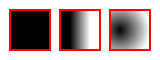
\includegraphics{graphics/gradients.pdf}

\hypertarget{flat-colored}{%
\paragraph{Flat Colored}\label{flat-colored}}

\begin{longtable}[]{@{}lll@{}}
\toprule
Field & Type & Description \\
\midrule
\endhead
color\_index & \texttt{VarUInt} & The index into the color table \\
\bottomrule
\end{longtable}

The shape is uniformly colored with the color at \texttt{color\_index}
in the color table.

\hypertarget{linear-gradient}{%
\paragraph{Linear Gradient}\label{linear-gradient}}

\begin{longtable}[]{@{}lll@{}}
\toprule
Field & Type & Description \\
\midrule
\endhead
point\_0 & \texttt{Point} & The start point of the gradient. \\
point\_1 & \texttt{Point} & The end point of the gradient. \\
color\_index\_0 & \texttt{VarUInt} & The color at \texttt{point\_0}. \\
color\_index\_1 & \texttt{VarUInt} & The color at \texttt{point\_1}. \\
\bottomrule
\end{longtable}

The gradient is formed by a mental line between \texttt{point\_0} and
\texttt{point\_1}. The color at \texttt{point\_0} is the color at
\texttt{color\_index\_0} in the color table, the color at
\texttt{point\_1} is the color at \texttt{color\_index\_1} in the color
table.

On the line, the color is linearly interpolated between the two points.
Each point that is not on the line is orthogonally projected to the line
and the color at that point is sampled. Points that are not projectable
onto the line have either the color at \texttt{point\_0} if they are
closed to \texttt{point\_0} or vice versa for \texttt{point\_1}.

\hypertarget{radial-gradient}{%
\paragraph{Radial Gradient}\label{radial-gradient}}

\begin{longtable}[]{@{}lll@{}}
\toprule
Field & Type & Description \\
\midrule
\endhead
point\_0 & \texttt{Point} & The start point of the gradient. \\
point\_1 & \texttt{Point} & The end point of the gradient. \\
color\_index\_0 & \texttt{VarUInt} & The color at \texttt{point\_0}. \\
color\_index\_1 & \texttt{VarUInt} & The color at \texttt{point\_1}. \\
\bottomrule
\end{longtable}

The gradient is formed by a mental circle with the center at
\texttt{point\_0} and \texttt{point\_1} being somewhere on the circle
outline. Thus, the radius of said circle is the distance between
\texttt{point\_0} and \texttt{point\_1}.

The color at \texttt{point\_0} is the color at \texttt{color\_index\_0}
in the color table, the color on the circle outline is the color at
\texttt{color\_index\_1} in the color table.

If a sampled point is inside the circle, a linear color interpolation is
done based on the distance to the center and the radius. If the point is
not in the circle itself, the color at \texttt{color\_index\_1} is
always taken.

\hypertarget{pathsegment_count}{%
\subsubsection{\texorpdfstring{\texttt{Path(segment\_count)}}{Path(segment\_count)}}\label{pathsegment_count}}

Paths describe instructions to create complex 2D graphics.

The mental model to form the path is this:\\
Each path segment generates a shape by moving a "pen" around. The path
this "pen" takes is the outline of our segment. Each segment, the "pen"
starts at a defined position and is moved by instructions. Each
instruction will leave the "pen" at a new position. The line drawn by
our "pen" is the outline of the shape.

The following instructions to move the "pen" are available:

\begin{longtable}[]{@{}lll@{}}
\toprule
Instruction Index & Instruction & Short Description \\
\midrule
\endhead
0 & line & A straight line is drawn from the current point to a new
point. \\
1 & horizontal line & A straight horizontal line is drawn from the
current point to a new \texttt{x} coordinate. \\
2 & vertical line & A straight vertical line is drawn from the current
point to a new \texttt{y} coordiante. \\
3 & cubic bezier & A cubic bezier curve is drawn from the current point
to a new point. \\
4 & arc circle & A circle segment is drawn from current point to a new
point. \\
5 & arc ellipse & An ellipse segment is drawn from current point to a
new point. \\
6 & close path & The path is closed and a straight line is drawn to the
starting point. \\
7 & quadratic bezier & A quadratic bezier curve is drawn from the
current point to a new point. \\
\bottomrule
\end{longtable}

As path encoding is hard to describe in a tabular manner, a verbal one
is chosen:

\begin{enumerate}
\def\labelenumi{\arabic{enumi}.}
\tightlist
\item
  For each segment in the path, the number of commands is encoded as a
  \texttt{VarUInt}.
\item
  For each segment in the path:

  \begin{enumerate}
  \def\labelenumii{\arabic{enumii}.}
  \tightlist
  \item
    A \texttt{Point} is encoded as the starting point.
  \item
    The instructions for this path, the number is determined in the
    first step.
  \item
    Each instruction is prefixed by a single tag byte that encodes the
    kind of instruction as well as the information if a line width is
    present.
  \item
    If a line width is present, that line width is read as a
    \texttt{Unit}
  \item
    The data for this command is decoded.
  \end{enumerate}
\end{enumerate}

The tag looks like this:

\begin{longtable}[]{@{}lll@{}}
\toprule
Field & Type & Description \\
\midrule
\endhead
instruction & \texttt{u3} & The instruction kind as listed in the table
above. \\
\emph{padding} & \texttt{u1} & Always 0 \\
has\_line\_width & \texttt{u1} & If \texttt{1}, a line width is
present. \\
\emph{padding} & \texttt{u3} & Always 0 \\
\bottomrule
\end{longtable}

\hypertarget{line-1}{%
\paragraph{Line}\label{line-1}}

The line instruction draws a straight line to the \texttt{position}.

\begin{longtable}[]{@{}lll@{}}
\toprule
Field & Type & Description \\
\midrule
\endhead
position & \texttt{Point} & The end point of the line. \\
\bottomrule
\end{longtable}

\hypertarget{horizontal-line}{%
\paragraph{Horizontal Line}\label{horizontal-line}}

The horizontal line instruction draws a straight horizontal line to a
given \texttt{x} coordinate.

\begin{longtable}[]{@{}lll@{}}
\toprule
Field & Type & Description \\
\midrule
\endhead
x & \texttt{Unit} & The new \texttt{x} coordinate. \\
\bottomrule
\end{longtable}

\hypertarget{vertical-line}{%
\paragraph{Vertical Line}\label{vertical-line}}

The vertical line instruction draws a straight vertical line to a given
\texttt{y} coordinate.

\begin{longtable}[]{@{}lll@{}}
\toprule
Field & Type & Description \\
\midrule
\endhead
y & \texttt{Unit} & The new \texttt{y} coordinate. \\
\bottomrule
\end{longtable}

\hypertarget{cubic-bezier}{%
\paragraph{Cubic Bezier}\label{cubic-bezier}}

The cubic bezier instruction draws a bézier curve with two control
points.

\begin{longtable}[]{@{}lll@{}}
\toprule
Field & Type & Description \\
\midrule
\endhead
control\_0 & \texttt{Point} & The first control point. \\
control\_1 & \texttt{Point} & The second control point. \\
point\_1 & \texttt{Point} & The end point of the bézier curve. \\
\bottomrule
\end{longtable}

The curve is drawn between the current location and \texttt{point\_1}
with \texttt{control\_0} being the first control point and
\texttt{control\_1} being the second one.

\hypertarget{arc-circle}{%
\paragraph{Arc Circle}\label{arc-circle}}

Draws a circle segment between the current and the \texttt{target}
point.

\begin{longtable}[]{@{}lll@{}}
\toprule
Field & Type & Description \\
\midrule
\endhead
large\_arc & \texttt{u1} & If \texttt{1}, the large portion of the
circle segment is drawn \\
sweep & \texttt{u1} & Determines if the circle segment is left- or right
bending. \\
\emph{padding} & \texttt{u6} & Always 0. \\
radius & \texttt{Unit} & The radius of the circle. \\
target & \texttt{Point} & The end point of the circle segment. \\
\bottomrule
\end{longtable}

\texttt{radius} determines the radius of the circle. If the distance
between the current point and \texttt{target} is larger than
\texttt{radius}, the distance is used as the radius.

When \texttt{large\_arc} is 1, the larger cirle segment is drawn.

If \texttt{sweep} is 1, the circle segment will make a left turn,
otherwise it will make a right turn. This means that if we go from the
current point to \texttt{target}, a rotation to the movement direction
is necessary to either the left or the right.

\hypertarget{arc-ellipse}{%
\paragraph{Arc Ellipse}\label{arc-ellipse}}

Draws an ellipse segment between the current and the \texttt{target}
point.

\begin{longtable}[]{@{}lll@{}}
\toprule
Field & Type & Description \\
\midrule
\endhead
large\_arc & \texttt{u1} & If \texttt{1}, the large portion of the
ellipse segment is drawn \\
sweep & \texttt{u1} & Determines if the ellipse segment is left- or
right bending. \\
\emph{padding} & \texttt{u6} & Always 0. \\
radius\_x & \texttt{Unit} & The radius of the ellipse in horizontal
direction. \\
radius\_y & \texttt{Unit} & The radius of the ellipse in vertical
direction. \\
rotation & \texttt{Unit} & The rotation of the ellipse in mathematical
negative direction, in degrees. \\
target & \texttt{Point} & The end point of ellipse circle segment. \\
\bottomrule
\end{longtable}

\texttt{radius\_x} and \texttt{radius\_y} determine the both radii of
the ellipse. If the distance between the current point and
\texttt{target} is not enough to fit any ellipse segment between the two
points, \texttt{radius\_x} and \texttt{radius\_y} are scaled uniformly
so that it fits exactly.

When \texttt{large\_arc} is 1, the larger cirle segment is drawn.

If \texttt{sweep} is 1, the ellipse segment will make a left turn,
otherwise it will make a right turn. This means that if we go from the
current point to \texttt{target}, a rotation to the movement direction
is necessary to either the left or the right.

\hypertarget{close-path}{%
\paragraph{Close Path}\label{close-path}}

A straight line is drawn to the start location of the current segment.
This instruction doesn't have additional data encoded.

\hypertarget{quadratic-bezier}{%
\paragraph{Quadratic Bezier}\label{quadratic-bezier}}

The quadratic bezier instruction draws a bézier curve with a single
control point.

\begin{longtable}[]{@{}lll@{}}
\toprule
Field & Type & Description \\
\midrule
\endhead
control & \texttt{Point} & The control point. \\
point\_1 & \texttt{Point} & The end point of the bézier curve. \\
\bottomrule
\end{longtable}

The curve is drawn between the current location and \texttt{point\_1}
with \texttt{control} being the control point.

\hypertarget{revision-history}{%
\subsection{Revision History}\label{revision-history}}

\hypertarget{10}{%
\subsubsection{1.0}\label{10}}

\begin{itemize}
\tightlist
\item
  Initial release
\end{itemize}

\end{document}
